\documentclass[aspectratio=43,11pt]{beamer}
\usetheme{default}
\usecolortheme{default}
\setbeamertemplate{navigation symbols}{}
\setbeamertemplate{footline}[frame number]
\setbeamertemplate{itemize items}[circle]
\usepackage{amsmath,amssymb,booktabs,tikz,pgfplots}
\pgfplotsset{compat=1.18}
\usetikzlibrary{arrows.meta,positioning,calc}
\definecolor{aggiemaroon}{RGB}{80,0,0}
\definecolor{deepblue}{RGB}{31,67,110}
\definecolor{midblue}{RGB}{36,110,170}
\definecolor{softgray}{RGB}{95,95,95}
\setbeamercolor{structure}{fg=aggiemaroon}
\setbeamercolor{frametitle}{fg=aggiemaroon}
\setbeamerfont{frametitle}{size=\large,series=\bfseries}
\setbeamertemplate{blocks}[rounded][shadow=false]
\title{Decision and Risk Analysis}
\subtitle{Lecture 10: \textbf{Why Hierarchical Models?}}
\author{Complete pooling, no pooling, and partial pooling}
\date{\color{aggiemaroon}{DAEN 427 / ISEN 427 / ISEN 627 - Fall 2026\\
      \textbf{Alexander Abuabara}}}
\titlegraphic{\vfill 
\includegraphics[height=1.2cm]{TAMU_logo.png}}

\begin{document}
\begin{frame}\titlepage\end{frame}

\begin{frame}{Learning goals}
\begin{itemize}
\item Recognize grouped or repeated-measures data.
\item Explain \textbf{complete pooling} and \textbf{no pooling}.
\item Identify limitations of both extremes.
\item Explain why \textbf{partial pooling} can improve inference and prediction.
\item Distinguish within-group from between-group variation.
\end{itemize}
\vspace{.5cm}
\textbf{Reading:} \emph{Bayes Rules!}, Chapter 15: 
\url{https://www.bayesrulesbook.com/chapter-15}
\end{frame}

\begin{frame}{A motivating question}
Suppose we measure the running time of the \emph{same people} in several races.
\begin{itemize}
\item Do all runners have the same typical time?
\item Does time change with age at the same rate for everyone?
\item Is one runner's 2024 time informative about their 2025 time?
\end{itemize}
\begin{block}{Key idea}
Observations can be related because they belong to the same person, school, laboratory, or other group.
\end{block}
\end{frame}

\begin{frame}{The Cherry Blossom race data}
\begin{itemize}
\item Annual 10-mile race in Washington, D.C.
\item \textbf{252 race results} from \textbf{36 runners}, each observed in multiple years.
\item Runners were in their 50s or 60s.
\item \(Y\): net finish time (minutes); \(X\): age (years).
\item \(j\) indexes runners; \(i\) indexes race results within runner.
\end{itemize}
\begin{block}{Question}
How does a runner's finishing time change as they age?
\end{block}
\end{frame}

\begin{frame}{What makes these data hierarchical?}
\centering
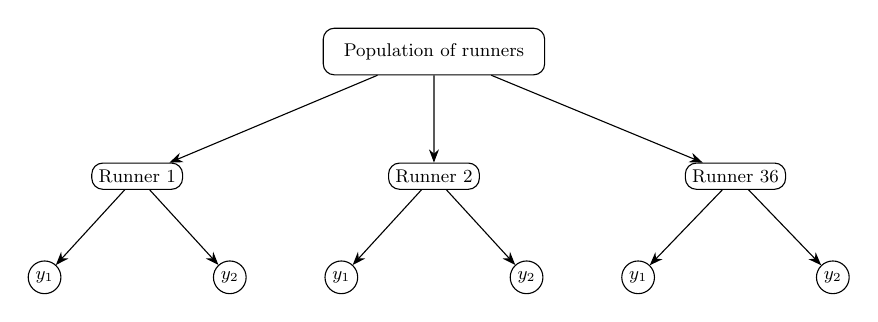
\begin{tikzpicture}[scale=0.74,transform shape,>=Stealth, node distance=9mm, every node/.style={font=\small}]
\node[draw,rounded corners,minimum width=38mm,minimum height=8mm] (pop) {Population of runners};
\node[draw,rounded corners,below left=15mm and 24mm of pop] (a) {Runner 1};
\node[draw,rounded corners,below=15mm of pop] (b) {Runner 2};
\node[draw,rounded corners,below right=15mm and 24mm of pop] (c) {Runner 36};
\draw[->] (pop)--(a); \draw[->](pop)--(b); \draw[->](pop)--(c);
\foreach \n in {a,b,c} {
 \node[draw,circle,inner sep=2pt,below left=13mm and 6mm of \n] (\n1) {$y_1$};
 \node[draw,circle,inner sep=2pt,below right=13mm and 6mm of \n] (\n2) {$y_2$};
 \draw[->](\n)--(\n1);\draw[->](\n)--(\n2);
}
\end{tikzpicture}
\vspace{3mm}
\begin{itemize}
\item \textbf{Between-runner} variation: typical times differ across runners.
\item \textbf{Within-runner} variation: times change across races for one runner.
\end{itemize}
\end{frame}

\begin{frame}{One runner's two observations}
For runner 1, the book reports:
\begin{center}
\begin{tabular}{ccc}\toprule Runner & Age & Time (min)\\\midrule 1 & 53 & 84.0\\ 1 & 54 & 74.3\\\bottomrule\end{tabular}
\end{center}
\begin{itemize}
\item Two results for the same runner need not be independent \emph{marginally}.
\item People have stable differences in ability and fitness.
\item Two points alone do not establish a long-term age trend.
\end{itemize}
\begin{block}{}
Would you treat these measurements as two unrelated people? Why not?
\end{block}
\end{frame}

\begin{frame}{Approach 1: Complete pooling}
\begin{block}{Strategy}
Put all 252 results together and fit \textbf{one regression line} for everyone.
\end{block}
\[
Y_i\mid\beta_0,\beta_1,\sigma\ \overset{\mathrm{ind}}\sim\
N(\beta_0+\beta_1 X_i,\sigma^2).
\]
\begin{itemize}
\item One intercept \(\beta_0\) and one age slope \(\beta_1\).
\item Runner identity does not appear in the model.
\item Assumes conditional independence of all observations given parameters.
\end{itemize}
\end{frame}

\begin{frame}{Complete pooling: what do we estimate?}
\begin{block}{Result reported in Chapter 15}
Posterior median age slope: \(\hat\beta_1 = 0.268\) minutes/year.
\[
80\%\text{ credible interval for }\beta_1:\quad [-0.302,\ 0.842].
\]
\end{block}
\begin{itemize}
\item The pooled relationship looks weak and uncertain.
\item The interval includes zero; the posterior does not establish a clear positive effect at this interval level.
\item But this pooled model may miss \emph{within-person} aging patterns.
\end{itemize}
\end{frame}

\begin{frame}{Illustration: many individual trends, one pooled trend}
\centering
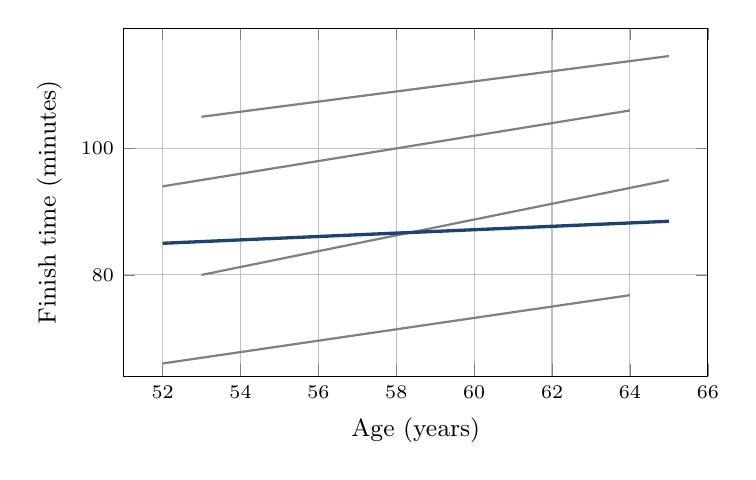
\begin{tikzpicture}
\begin{axis}[width=9cm,height=6cm,xlabel={Age (years)},ylabel={Finish time (minutes)},xmin=51,xmax=66,ymin=64,ymax=119,grid=major,tick label style={font=\scriptsize},label style={font=\small}]
\addplot[gray,thick,domain=52:64] {66+0.9*(x-52)};
\addplot[gray,thick,domain=53:65] {80+1.25*(x-53)};
\addplot[gray,thick,domain=52:64] {94+1.0*(x-52)};
\addplot[gray,thick,domain=53:65] {105+0.8*(x-53)};
\addplot[deepblue,very thick,domain=52:65] {85+0.268*(x-52)};
\end{axis}
\end{tikzpicture}
\vspace{-1mm}
{\scriptsize Schematic trends, \textbf{not} a reconstruction of the dataset.\\
             Gray: individuals; blue: pooled.}
\end{frame}

\begin{frame}{Why complete pooling can fail}
\begin{enumerate}
\item \textbf{Dependence:} observations from one runner share runner-specific characteristics.
\item \textbf{Heterogeneity:} different runners have different starting levels and potentially different age slopes.
\end{enumerate}
\begin{block}{Important distinction}
A weak \emph{cross-sectional} age trend does not imply that a person's time barely changes \emph{as that person ages}.
\end{block}
\begin{itemize}
\item Ignoring the group structure can distort uncertainty and conclusions.
\item This is a modeling issue, not a failure of Bayesian statistics.
\end{itemize}
\end{frame}

\begin{frame}{Approach 2: No pooling}
\begin{block}{Strategy}
Fit a \textbf{separate regression} to every runner.
\end{block}
\[
Y_{ij}\mid\beta_{0j},\beta_{1j},\sigma\sim
N(\beta_{0j}+\beta_{1j}X_{ij},\sigma^2).
\]
\begin{itemize}
\item Runner \(j\) has their own intercept \(\beta_{0j}\).
\item Runner \(j\) has their own slope \(\beta_{1j}\).
\item No group-level structure connects the regression coefficients across runners.
\end{itemize}
\end{frame}

\begin{frame}{No pooling: runner 1 thought experiment}
\begin{itemize}
\item Runner 1 has only about five observed races (book).
\item A separately fitted line suggests that this runner becomes faster with age.
\item Extrapolating that line can produce an implausibly fast prediction at age 62.
\end{itemize}
\begin{block}{Think--pair--share}
Should we trust one runner's downward-sloping line, or use information from the other 35 runners as well?
\end{block}
\end{frame}

\begin{frame}{Why no pooling can fail}
\begin{enumerate}
\item \textbf{Small groups are noisy:} a slope based on five results may be unstable.
\item \textbf{No borrowing of information:} trends from other runners cannot help estimate this runner's trend.
\item \textbf{New groups:} there is no fitted group-specific line for a runner never observed before.
\end{enumerate}
\begin{block}{Tradeoff}
More flexibility is not automatically better prediction.
\end{block}
\end{frame}

\begin{frame}{Approach 3: Partial pooling}
\begin{block}{Strategy}
Give each runner their own trend, \textbf{but connect those trends through a shared population distribution}.
\end{block}
\begin{itemize}
\item Runners may differ in average time and rate of aging.
\item Evidence from all runners informs population-level patterns.
\item Group-specific estimates are \emph{partly pulled} toward a common pattern.
\item This regularization is often called \textbf{shrinkage}.
\end{itemize}
\end{frame}

\begin{frame}{A preview of a hierarchical model}
\textbf{Observation level:}
\[
Y_{ij}\mid\beta_{0j},\beta_{1j},\sigma\sim
N(\beta_{0j}+\beta_{1j}X_{ij},\sigma^2).
\]
\textbf{Runner level:} {\tiny (illustrative specification)}
\[
\begin{pmatrix}\beta_{0j}\\\beta_{1j}\end{pmatrix}
\sim N_2\!\left(\begin{pmatrix}\mu_0\\\mu_1\end{pmatrix},\Sigma\right).
\]
\begin{itemize}
\item \((\mu_0,\mu_1)\): population-average coefficients.
\item \(\Sigma\): between-runner variation and association in coefficients.
\item Priors on population parameters complete the Bayesian model.
\end{itemize}
{\scriptsize Preview: Chapter 15 motivates this model; later chapters develop it.}
\end{frame}

\begin{frame}{Visual intuition: shrinkage}
\begin{center}
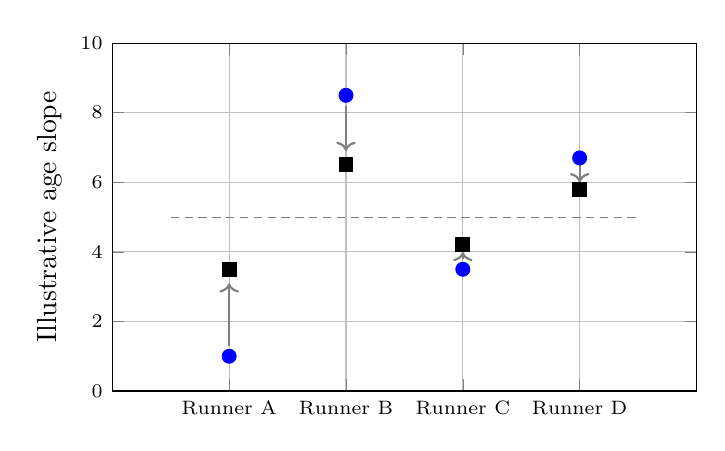
\begin{tikzpicture}
\begin{axis}[width=9cm,height=6cm,xmin=0,xmax=5,ymin=0,ymax=10,xtick={1,2,3,4},xticklabels={Runner A,Runner B,Runner C,Runner D},ylabel={Illustrative age slope},xlabel={},grid=major,tick label style={font=\scriptsize}]
\addplot[only marks,mark=*,mark size=2.5pt,blue] coordinates {(1,1)(2,8.5)(3,3.5)(4,6.7)};
\addplot[only marks,mark=square*,mark size=2.5pt,black] coordinates {(1,3.5)(2,6.5)(3,4.2)(4,5.8)};
\addplot[densely dashed,gray,domain=0.5:4.5] {5};
\draw[->,thick,gray] (axis cs:1,1.3)--(axis cs:1,3.1);
\draw[->,thick,gray] (axis cs:2,8.2)--(axis cs:2,6.9);
\draw[->,thick,gray] (axis cs:3,3.8)--(axis cs:3,4.0);
\draw[->,thick,gray] (axis cs:4,6.5)--(axis cs:4,6.0);
\end{axis}
\end{tikzpicture}
\end{center}
{Schematic illustration only:\\
- Blue dots: no-pooling estimates;\\
- Black squares: partial-pooling estimates;\\
- Dashed: shared population tendency.}
\end{frame}

\begin{frame}{How much pooling?}
\begin{itemize}
\item \textbf{Little data for a runner}: individual estimate tends to be more uncertain and often shrinks more.
\item \textbf{Lots of precise data for a runner}: its own data may dominate, so shrinkage is smaller.
\item \textbf{Runners are similar}: pooling is often stronger.
\item \textbf{Runners are very different}: pooling may be weaker.
\end{itemize}
\begin{block}{Intuition}
Partial pooling learns the strength of sharing from the data and model rather than forcing everyone to be identical.
\end{block}
\end{frame}

\begin{frame}{Comparison: all three approaches}
\small
\begin{tabular}{p{2.7cm}p{2.4cm}p{4.4cm}}
\toprule
 & Runner-specific? & Shares information across runners?\\\midrule
Complete pooling & No & Yes; forces one common line\\[2mm]
No pooling & Yes & No\\[2mm]
Partial pooling & Yes & Yes; estimates related through population model\\
\bottomrule
\end{tabular}
\vspace{7mm}
\begin{block}{In one-sentence ...}
Complete pooling ignores differences;\\
\qquad no pooling ignores similarities;\\
\qquad \qquad partial pooling models both.
\end{block}
\end{frame}

\begin{frame}{Predicting a brand-new runner}
Imagine a runner not among the original 36.
\begin{itemize}
\item \textbf{Complete pooling:} use the one universal line; may miss aging patterns.
\item \textbf{No pooling:} no estimated line exists for this new runner.
\item \textbf{Partial pooling:} use the learned population distribution to describe a new runner's possible intercept and slope.
\end{itemize}
\begin{block}{Question:}
Why should a prediction for a new runner include \emph{between-runner} uncertainty?
\end{block}
\end{frame}

\begin{frame}{Example beyond running: schools}
We collect test scores from several students within each school.
\begin{itemize}
\item \textbf{Groups:} schools.
\item \textbf{Observations:} students within schools.
\item \textbf{Within-school variability:} students at one school have different scores.
\item \textbf{Between-school variability:} schools differ in typical scores.
\end{itemize}
\begin{block}{Question}
Suppose one school has only three sampled students. How might information from other schools improve estimation?
\end{block}
\end{frame}

\begin{frame}[fragile]{R: explore grouping!}
\scriptsize
\begin{verbatim}
library(bayesrules)
library(dplyr)
library(ggplot2)

data(cherry_blossom_sample)
running <- cherry_blossom_sample |>
  select(runner, age, net)

# See how finish times vary by runner
ggplot(running, aes(runner, net)) +
  geom_boxplot() +
  labs(x = "Runner", y = "Finish time (min)")

# Compare within-runner patterns
ggplot(running, aes(age, net, group = runner)) +
  geom_point(alpha = 0.5) +
  geom_smooth(method = "lm", se = FALSE)
\end{verbatim}
\end{frame}

\begin{frame}{Check}
For each situation, choose the modeling concern.
\begin{enumerate}
\item A model assumes every school has the same mean score.
\item A model estimates a separate slope from just two observations per person.
\item A model estimates separate slopes but learns a shared population trend.
\end{enumerate}
\vspace{5mm}
\textbf{Choices:} complete pooling, no pooling, partial pooling.
\end{frame}

\begin{frame}{Answers and takeaways}
\begin{enumerate}
\item \textbf{Complete pooling}: may hide differences among schools.
\item \textbf{No pooling}: group estimates may be unstable with little data.
\item \textbf{Partial pooling}: allows variation while sharing information.
\end{enumerate}
\vspace{5mm}
\begin{block}{Remember}
Grouped data call for models that respect the groups. Partial pooling provides a principled compromise between one-size-fits-all and completely separate analyses.
\end{block}
\end{frame}

\begin{frame}{Possible questions/questions to practice}
\begin{enumerate}
\item Give an example of data with observations nested within groups.
\item Define \emph{within-group} and \emph{between-group} variation in your example.
\item Explain, in two sentences, why partial pooling may be preferable to both extremes.
\end{enumerate}
\end{frame}
\end{document}